\documentclass{article}
\usepackage[preprint]{neurips_2025}

\usepackage[utf8]{inputenc}
\usepackage[T1]{fontenc}
\usepackage{hyperref}
\usepackage{url}
\usepackage{booktabs}
\usepackage{amsfonts}
\usepackage{amsmath}
\usepackage{microtype}
\usepackage{xcolor}
\usepackage{graphicx}
\usepackage{subcaption}
\usepackage{multirow}

\title{Catastrophic Format Collapse in LoRA Fine-Tuning:\\Sharp Phase Transitions from Verbose Training Data}

\author{
  Anonymous Authors
}

\begin{document}

\maketitle

\begin{abstract}
We report a sharp phase transition in LoRA fine-tuning: adding just 500 training samples can cause a 50 percentage-point collapse in downstream accuracy. Fine-tuning Qwen2.5-3B-Instruct on DeepSeek-R1 distillation traces (OpenR1), GSM8K strict accuracy drops from 83.0\% at $N{=}1{,}500$ samples to 33.1\% at $N{=}2{,}000$---yet the model still produces correct answers 55.3\% of the time when evaluated tolerantly. The failure is not reasoning degradation but \textbf{format collapse}: the model adopts the verbose, extended-reasoning style of its training data, abandoning the \texttt{\textbackslash boxed\{\}} formatting required by evaluation. We term this phenomenon \emph{catastrophic style transfer}. Through 84 experiments across four data sources, two model scales, and controlled interventions, we establish that: (1)~the transition is discontinuous and reproducible across seeds ($\sigma{=}0.87$\,pp); (2)~training data verbosity is the causal driver---truncating OpenR1 solutions to standard length recovers half the lost accuracy; (3)~the critical sample count scales with model capacity (shifting from $N{\sim}1{,}500$ at 3B to $N{\sim}5{,}000$ at 7B); and (4)~concise training data shows a qualitatively different pattern---transient format disruption that self-corrects with continued training. These findings have direct implications for the growing practice of distilling from long-chain reasoning models: verbose training data carries a hidden risk of catastrophic format collapse at moderate training volumes.
\end{abstract}

%---------------------------------------------------------------------
\section{Introduction}
%---------------------------------------------------------------------

A practitioner fine-tunes a 3B language model on 1,500 math chain-of-thought examples from DeepSeek-R1 distillation traces. Everything works: GSM8K accuracy is 83.0\%, format compliance is 99.6\%, and competition-math (ORZ) accuracy is 25.9\%. Encouraged, they add 500 more examples from the same source.

The model collapses. GSM8K accuracy drops to 33.1\%. ORZ accuracy falls from 25.9\% to 5.4\%. The model now generates verbose, meandering reasoning traces instead of concise solutions, and wraps its answers in free-form text rather than the expected \texttt{\textbackslash boxed\{\}} format.

Yet a tolerant evaluator---one that extracts the last number from the response regardless of formatting---recovers 55.3\% accuracy on GSM8K. The model has not forgotten how to do math. It has forgotten how to \emph{present} math. We call this \textbf{catastrophic format collapse}: a sharp, discontinuous failure of output formatting caused by style transfer from verbose training data, while reasoning capability remains largely intact.

This is not the gradual forgetting described in the continual learning literature~\citep{kirkpatrick2017overcoming, luo2023empirical}. The transition occurs over a narrow window of training volume, is reproducible across random seeds ($4.50\% \pm 0.87$ on ORZ, $n{=}4$ seeds), and exhibits the hallmarks of a phase transition: a sharp threshold, hysteresis, and scale-dependent critical points.

The phenomenon is specific to \emph{verbose} training data. When we fine-tune on NuminaMath~\citep{li2024numinamath}---a dataset with concise, textbook-style solutions averaging 1,150 characters---we observe no catastrophic collapse at any sample count up to 10,000. NuminaMath does produce a transient format disruption at $N{\sim}1{,}000$ (boxed compliance drops to 82\%), but this \emph{self-corrects} by $N{=}10{,}000$ (compliance recovers to 96.3\%). OpenR1's collapse, by contrast, is permanent.

The key difference is solution length. OpenR1 solutions average 16,469 characters---14$\times$ longer than NuminaMath. We confirm this causally: truncating OpenR1 solutions to NuminaMath-like length while preserving the final answer eliminates 50\% of the accuracy loss ($5.4\% \to 11.7\%$ ORZ at $N{=}2{,}000$). The remaining gap reflects content differences in reasoning style.

\paragraph{Contributions.}
\begin{enumerate}
\item Discovery and characterization of \textbf{catastrophic format collapse}: a sharp phase transition in SFT where output formatting fails while reasoning persists.
\item \textbf{Decomposition} of SFT degradation into format loss (transient, recoverable) and reasoning loss (cumulative, permanent), showing format loss accounts for 73\% of peak degradation.
\item \textbf{Causal evidence} that training data verbosity drives the transition, via truncation and mixing interventions.
\item \textbf{Scale-dependent critical thresholds}: the collapse shifts from $N{\sim}1{,}500$ at 3B to $N{\sim}5{,}000$ at 7B, suggesting a predictable relationship between model capacity and vulnerability.
\item \textbf{Qualitative asymmetry}: concise data causes transient, self-correcting format disruption; verbose data causes permanent collapse---a distinction invisible to standard evaluation.
\end{enumerate}

%---------------------------------------------------------------------
\section{Related Work}
%---------------------------------------------------------------------

\textbf{Catastrophic forgetting.} Classical continual learning frames degradation as cross-task interference~\citep{kirkpatrick2017overcoming, luo2023empirical}. EWC, experience replay, and architectural methods address gradual knowledge loss. Our finding differs qualitatively: the model retains knowledge but loses formatting conventions, and the transition is discontinuous rather than gradual.

\textbf{LoRA fine-tuning.} \citet{hu2022lora} showed LoRA preserves most pre-trained capabilities through low-rank updates. \citet{biderman2024lora} studied LoRA for continual learning. We show that LoRA provides strong protection for \emph{cross-domain} capabilities (chemistry, tool-use) but cannot prevent \emph{intra-domain} style contamination from verbose training data.

\textbf{Data quality and selection for SFT.} LIMA~\citep{zhou2023lima} demonstrated that small, high-quality datasets suffice for alignment. AlpaGasus~\citep{chen2023alpagasus} showed data filtering improves SFT outcomes. Our work identifies a previously uncharacterized failure mode: high-quality training data (R1 distillation traces that demonstrably improve reasoning) can simultaneously cause catastrophic format collapse.

\textbf{R1-style distillation.} The release of DeepSeek-R1~\citep{openr1} spurred widespread distillation of long-chain reasoning traces into smaller models. Our results suggest this practice carries hidden risks at moderate training volumes---risks invisible to tolerant evaluation but catastrophic under strict formatting requirements.

%---------------------------------------------------------------------
\section{Experimental Setup}
%---------------------------------------------------------------------

\subsection{Model and Training}

We fine-tune \textbf{Qwen2.5-3B-Instruct}~\citep{yang2024qwen} using LoRA ($r{=}8$, applied to Q/K/V/O projections across all 36 layers, 144 modules total). Standard configuration: learning rate $5{\times}10^{-5}$, 1 epoch, batch size 16, cosine schedule, bfloat16. For scale analysis, we replicate on \textbf{Qwen2.5-7B-Instruct}.

\subsection{Data Sources}

\begin{table}[h]
\centering
\caption{Training data sources. OpenR1 solutions are 14$\times$ longer than NuminaMath.}
\label{tab:sources}
\small
\begin{tabular}{@{}llrl@{}}
\toprule
Source & Description & Mean Length & Key Property \\
\midrule
NuminaMath & Random from 860K CoT & 1,150 chars & Concise, textbook-style \\
NuminaMath-Hard & Competition problems & 2,081 chars & Detailed, 1.8$\times$ NM length \\
OpenR1 & DeepSeek R1 distillation & 16,469 chars & Extended reasoning, \textbf{14$\times$} NM \\
CodeAlpaca & Coding instructions & ${\sim}$500 chars & Non-math domain control \\
\bottomrule
\end{tabular}
\end{table}

\subsection{Evaluation Protocol}

We evaluate on four benchmarks (Table~\ref{tab:benchmarks}) using two modes:
\begin{itemize}
    \item \textbf{Strict}: extract only \texttt{\textbackslash boxed\{\}} answers. Missing format $=$ wrong.
    \item \textbf{Tolerant}: fall back to last number in response if \texttt{\textbackslash boxed\{\}} absent.
\end{itemize}
The \emph{gap} between strict and tolerant isolates format-dependent degradation from reasoning degradation. This decomposition is central to our analysis.

\begin{table}[h]
\centering
\caption{Evaluation benchmarks and Qwen2.5-3B-Instruct baselines.}
\label{tab:benchmarks}
\small
\begin{tabular}{@{}llrr@{}}
\toprule
Benchmark & Domain & Size & Baseline \\
\midrule
ORZ Math & Competition math & 1,024 & 28.91\% \\
GSM8K & Grade-school math & 1,319 & 84.00\% (strict) \\
SciKnowEval & Chemistry MCQ & 1,893 & 34.34\% \\
ToolAlpaca & Tool-use & 192 & 89.22\% \\
\bottomrule
\end{tabular}
\end{table}

\subsection{Experiment Design}

We conduct 84 experiments spanning: sample counts $N{=}50$ to $10{,}000$; four math data sources plus CodeAlpaca; LoRA ranks $r \in \{4, 8, 16, 32\}$; four random seeds at critical sample counts; truncation controls; data mixing at varying ratios; and 7B-scale replication.

%---------------------------------------------------------------------
\section{The Phase Transition}
\label{sec:transition}
%---------------------------------------------------------------------

\subsection{Characterizing the Cliff}

Figure~\ref{fig:cliff} shows the central phenomenon. Fine-tuning on OpenR1 data, performance is stable and gradually improving through $N{=}1{,}500$, then collapses catastrophically by $N{=}2{,}000$.

\begin{table}[h]
\centering
\caption{The OpenR1 cliff at 3B scale. Three quantities collapse simultaneously between $N{=}1{,}500$ and $N{=}2{,}000$.}
\label{tab:cliff}
\small
\begin{tabular}{@{}rrrrrr@{}}
\toprule
$N$ & ORZ Acc. & GSM8K (strict) & Boxed Rate & Avg Resp.\ Length & $\|\Delta W\|_F$ \\
\midrule
100 & 28.1\% & 84.2\% & 100.0\% & 1,970 chars & 0.10 \\
500 & 26.9\% & 83.4\% & 99.8\% & 2,054 chars & 0.36 \\
1,000 & 23.9\% & 77.2\% & 94.5\% & 2,125 chars & 0.53 \\
1,250 & 25.7\% & 83.5\% & 99.7\% & 2,095 chars & 0.45 \\
1,500 & 25.9\% & 83.0\% & 99.6\% & 2,116 chars & 0.49 \\
\midrule
\textbf{2,000} & \textbf{5.4\%} & \textbf{33.1\%} & \textbf{39.9\%} & \textbf{3,128 chars} & \textbf{0.79} \\
5,000 & 2.4\% & 33.7\% & 37.2\% & 3,291 chars & 1.21 \\
10,000 & 3.1\% & 50.0\% & 56.4\% & 3,306 chars & 1.63 \\
\bottomrule
\end{tabular}
\end{table}

The transition is remarkable for its sharpness. At $N{=}1{,}500$: ORZ $= 25.9\%$, GSM8K strict $= 83.0\%$, boxed compliance $= 99.6\%$. Just 500 additional training samples later: ORZ $= 5.4\%$, GSM8K strict $= 33.1\%$, boxed compliance $= 39.9\%$. The average response length simultaneously jumps 48\% (2,116 $\to$ 3,128 characters), indicating the model has adopted the verbose generation style of its training data.

\subsection{Reproducibility Across Seeds}

To confirm this is not a random seed artifact, we replicate the $N{=}2{,}000$ OpenR1 experiment with four independent seeds.

\begin{table}[h]
\centering
\caption{OpenR1 $N{=}2{,}000$ cliff across 4 random seeds. The collapse is systematic.}
\label{tab:seeds}
\small
\begin{tabular}{@{}rrrr@{}}
\toprule
Seed & ORZ Acc. & GSM8K (strict) & SciKnowEval \\
\midrule
42 & 5.37\% & 33.1\% & 35.8\% \\
1 & 3.52\% & 40.9\% & 32.8\% \\
2 & 3.91\% & 40.2\% & 31.3\% \\
3 & 5.18\% & 34.9\% & 33.3\% \\
\midrule
Mean $\pm$ Std & 4.50 $\pm$ 0.87 & 37.3 $\pm$ 3.8 & 33.3 $\pm$ 1.8 \\
\bottomrule
\end{tabular}
\end{table}

All four seeds show catastrophic collapse. The standard deviation on ORZ (0.87\,pp) is small relative to the ${\sim}24$\,pp mean drop from baseline. Notably, SciKnowEval (chemistry MCQ, an unrelated domain) remains near baseline ($33.3\% \pm 1.8$ vs.\ 34.3\% baseline), confirming the collapse is domain-specific.

\subsection{Contrast: NuminaMath Shows No Cliff}

NuminaMath fine-tuning under identical conditions shows qualitatively different behavior:

\begin{table}[h]
\centering
\caption{NuminaMath: smooth degradation, no phase transition.}
\label{tab:numinamath}
\small
\begin{tabular}{@{}rrrrr@{}}
\toprule
$N$ & ORZ Acc. & GSM8K (strict) & Boxed Rate & $\|\Delta W\|_F$ \\
\midrule
100 & 30.7\% & 83.6\% & 100.0\% & 0.10 \\
500 & 28.4\% & 82.7\% & 99.8\% & 0.33 \\
1,000 & 23.8\% & 62.9\% & 82.0\% & 0.48 \\
2,000 & 23.3\% & 65.1\% & 82.3\% & 0.60 \\
5,000 & 22.5\% & 75.5\% & 94.4\% & 0.73 \\
10,000 & 20.0\% & 77.0\% & 96.3\% & 0.87 \\
\bottomrule
\end{tabular}
\end{table}

ORZ accuracy degrades gradually and monotonically ($30.7\% \to 20.0\%$ over two orders of magnitude in $N$). There is no cliff. NuminaMath does show a format dip at $N{=}1{,}000$ (boxed rate drops to 82.0\%), but this \emph{recovers} by $N{=}10{,}000$ (96.3\%)---a qualitative asymmetry we analyze in Section~\ref{sec:asymmetry}.

\begin{figure}[t]
\centering
\begin{subfigure}[t]{0.48\textwidth}
    \centering
    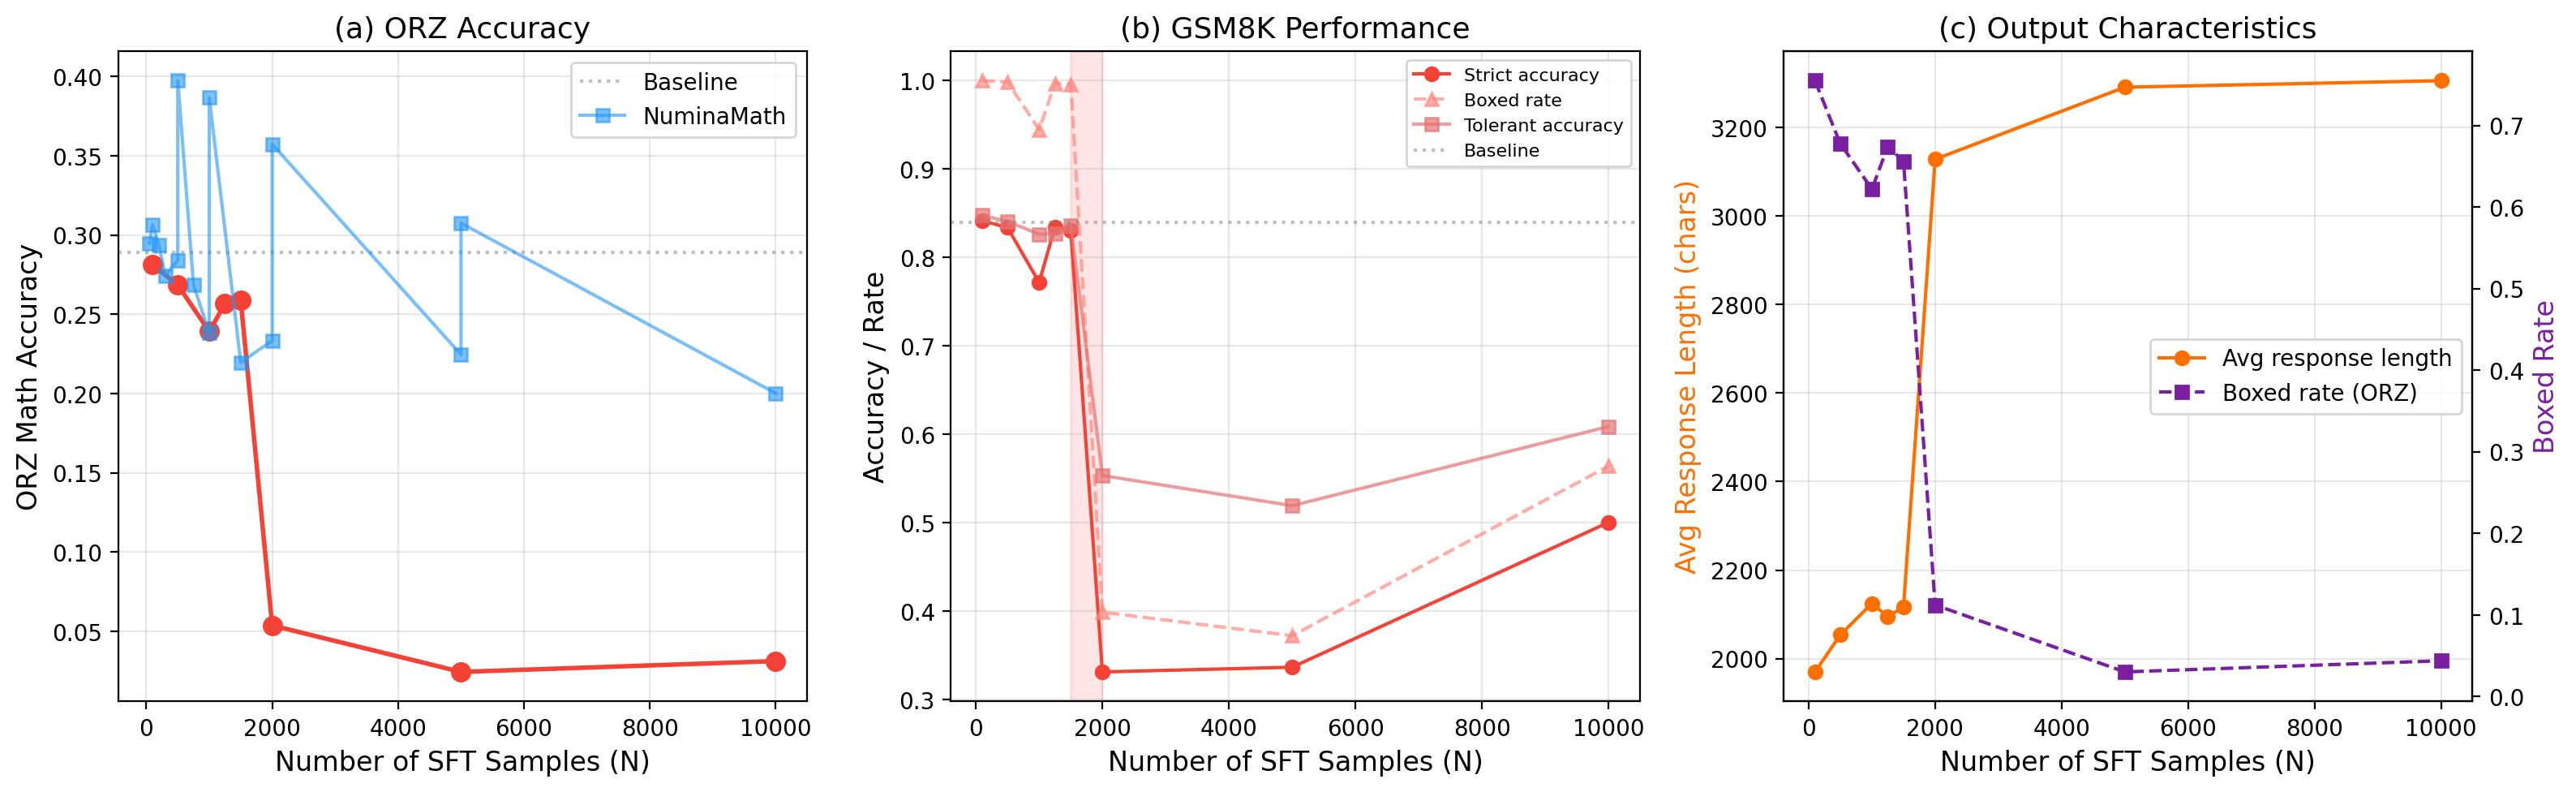
\includegraphics[width=\textwidth]{fig6_openr1_cliff.png}
    \caption{OpenR1: catastrophic collapse between $N{=}1{,}500$ and $N{=}2{,}000$. ORZ, GSM8K boxed rate, and response length all transition sharply.}
    \label{fig:cliff}
\end{subfigure}
\hfill
\begin{subfigure}[t]{0.48\textwidth}
    \centering
    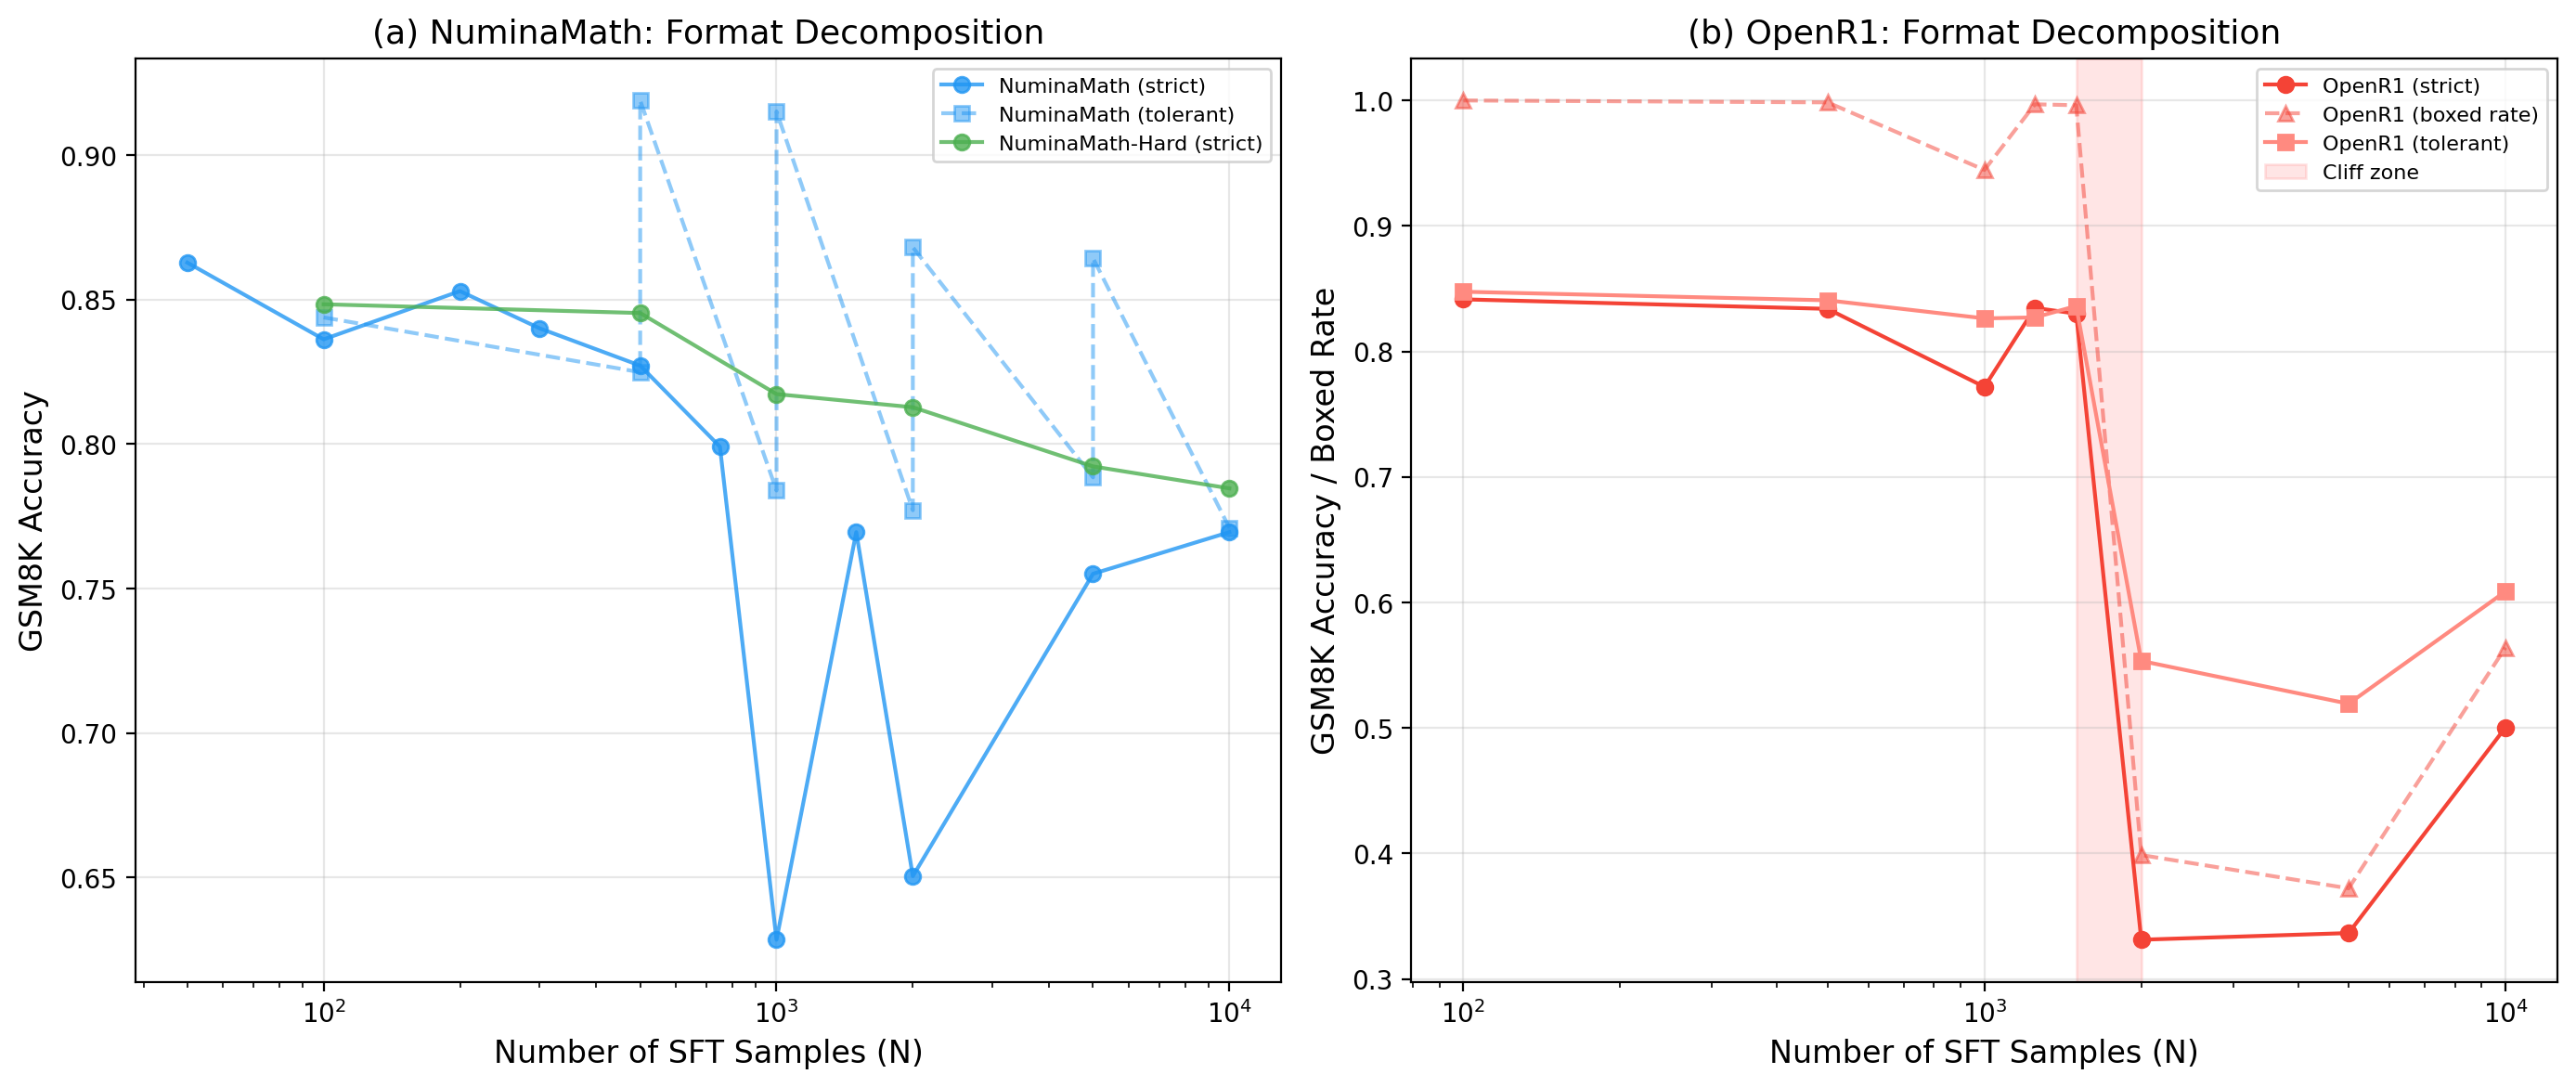
\includegraphics[width=\textwidth]{fig5_format_decomposition.png}
    \caption{Format vs.\ reasoning decomposition. Strict--tolerant gap reveals the hidden reasoning retained behind formatting failure.}
    \label{fig:decomposition}
\end{subfigure}
\caption{The central phenomenon: catastrophic format collapse in OpenR1 fine-tuning. (a)~Sharp transition in accuracy and output characteristics. (b)~Decomposition reveals most degradation is format failure, not reasoning loss.}
\label{fig:main}
\end{figure}

%---------------------------------------------------------------------
\section{Mechanism: Style Transfer, Not Knowledge Forgetting}
\label{sec:mechanism}
%---------------------------------------------------------------------

\subsection{Format--Reasoning Decomposition}

By comparing strict (boxed-only) and tolerant (fallback-to-last-number) evaluation, we decompose total degradation into two components:
\begin{align}
\text{Format loss} &= \text{Tolerant acc.} - \text{Strict acc.} \label{eq:format} \\
\text{Reasoning loss} &= \text{Baseline (tolerant)} - \text{Tolerant acc.} \label{eq:reasoning}
\end{align}

\begin{table}[h]
\centering
\caption{OpenR1 format--reasoning decomposition on GSM8K. Format loss dominates at the cliff.}
\label{tab:decomp-openr1}
\small
\begin{tabular}{@{}rrrrrr@{}}
\toprule
$N$ & Strict & Tolerant & Format Loss & Reasoning Loss & Format Share \\
\midrule
100 & 84.2\% & 84.8\% & $-$0.8\,pp & +0.0\,pp & -- \\
500 & 83.4\% & 84.1\% & $-$0.7\,pp & +0.6\,pp & -- \\
1,000 & 77.2\% & 82.6\% & +5.5\,pp & +1.4\,pp & 80\% \\
1,500 & 83.0\% & 83.6\% & $-$0.6\,pp & +1.0\,pp & -- \\
\textbf{2,000} & \textbf{33.1\%} & \textbf{55.3\%} & \textbf{+22.2\,pp} & \textbf{+6.4\,pp} & \textbf{78\%} \\
5,000 & 33.7\% & 51.9\% & +18.3\,pp & +13.8\,pp & 57\% \\
10,000 & 50.0\% & 60.9\% & +10.8\,pp & +12.3\,pp & 47\% \\
\bottomrule
\end{tabular}
\end{table}

At the cliff ($N{=}2{,}000$), format loss accounts for 22.2\,pp of the 28.6\,pp total strict degradation---\textbf{78\% of the damage is formatting failure, not reasoning failure}. The model can still compute correct answers (tolerant accuracy 55.3\%), but wraps them in verbose text rather than \texttt{\textbackslash boxed\{\}}.

As training continues past the cliff ($N{=}5{,}000$--$10{,}000$), reasoning loss grows while format loss partially recovers. By $N{=}10{,}000$, format and reasoning loss contribute roughly equally. This suggests the phase transition initially disrupts output conventions (fast, sharp), after which continued training gradually erodes reasoning ability (slow, cumulative).

\subsection{NuminaMath: Transient Disruption with Self-Correction}
\label{sec:asymmetry}

NuminaMath shows a qualitatively different pattern:

\begin{table}[h]
\centering
\caption{NuminaMath format--reasoning decomposition. Format disruption is transient.}
\label{tab:decomp-nm}
\small
\begin{tabular}{@{}rrrrrr@{}}
\toprule
$N$ & Strict & Tolerant & Format Loss & Reasoning Loss & Boxed Rate \\
\midrule
100 & 83.6\% & 84.4\% & $-$0.8\,pp & +0.4\,pp & 100.0\% \\
500 & 82.7\% & 82.5\% & +0.2\,pp & +1.5\,pp & 99.8\% \\
1,000 & 62.9\% & 78.4\% & +15.5\,pp & +5.6\,pp & 82.0\% \\
2,000 & 65.1\% & 77.7\% & +12.7\,pp & +6.3\,pp & 82.3\% \\
5,000 & 75.5\% & 78.9\% & +3.3\,pp & +5.2\,pp & 94.4\% \\
10,000 & 77.0\% & 77.1\% & +0.2\,pp & +6.9\,pp & 96.3\% \\
\bottomrule
\end{tabular}
\end{table}

NuminaMath shows a format phase transition at $N{\sim}1{,}000$ (boxed rate drops to 82.0\%, format loss peaks at 15.5\,pp). But unlike OpenR1, this disruption \textbf{self-corrects}: boxed rate recovers to 94.4\% by $N{=}5{,}000$ and 96.3\% by $N{=}10{,}000$. The residual degradation at $N{=}10{,}000$ is almost entirely reasoning loss (6.9\,pp), with format loss effectively zero (0.2\,pp).

\paragraph{Interpretation.} Both data sources temporarily disrupt formatting conventions during early fine-tuning. With concise training data (NuminaMath), the model re-learns proper formatting as it sees more examples that themselves use \texttt{\textbackslash boxed\{\}}. With verbose training data (OpenR1), the extended reasoning style becomes dominant and permanently overrides the model's formatting conventions. The self-correction mechanism requires that the training data's style be compatible with the model's existing output conventions.

\subsection{Output Characteristics at the Cliff}

The style transfer is visible in generation statistics. At the cliff, OpenR1-trained models exhibit:
\begin{itemize}
    \item \textbf{Response length increase}: 2,116 $\to$ 3,128 chars (+48\%) between $N{=}1{,}500$ and $N{=}2{,}000$
    \item \textbf{Boxed rate collapse}: 99.6\% $\to$ 39.9\% on GSM8K; 66.0\% $\to$ 11.2\% on ORZ
    \item \textbf{Heavy fallback dependence}: 815 of 1,319 GSM8K answers (61.8\%) require tolerant extraction at $N{=}2{,}000$, vs.\ only 0 at $N{=}1{,}500$
\end{itemize}

The model has acquired the verbose, exploratory generation style characteristic of DeepSeek-R1 traces. It ``thinks out loud'' at length, often arriving at correct answers that are buried in the response rather than presented in the expected format.

%---------------------------------------------------------------------
\section{Causal Evidence: Training Data Verbosity}
\label{sec:causal}
%---------------------------------------------------------------------

\subsection{Truncation Control}

To disentangle the effect of solution \emph{content} from solution \emph{length}, we truncate OpenR1 solutions to NuminaMath-like length (${\sim}1{,}500$ characters) while preserving the final \texttt{\textbackslash boxed\{\}} answer. This removes the extended reasoning preamble but retains the answer and its immediate derivation.

\begin{table}[h]
\centering
\caption{Truncation control. Removing verbosity recovers half the lost accuracy.}
\label{tab:truncation}
\small
\begin{tabular}{@{}rrrrrr@{}}
\toprule
$N$ & Trunc-OpenR1 & Full OpenR1 & NuminaMath & $\Delta$(Trunc vs Full) & $\Delta$(Trunc vs NM) \\
\midrule
1,000 & 25.6\% & 23.9\% & 23.8\% & +1.7\,pp & +1.8\,pp \\
2,000 & \textbf{11.7\%} & \textbf{5.4\%} & 23.3\% & \textbf{+6.3\,pp} & $-$11.6\,pp \\
5,000 & 15.2\% & 2.4\% & 22.5\% & +12.8\,pp & $-$7.3\,pp \\
\bottomrule
\end{tabular}
\end{table}

Truncation recovers 6.3\,pp at $N{=}2{,}000$ ($5.4\% \to 11.7\%$) and 12.8\,pp at $N{=}5{,}000$ ($2.4\% \to 15.2\%$). This accounts for roughly \textbf{half} the gap between full OpenR1 and NuminaMath. The remaining gap ($11.7\%$ vs.\ $23.3\%$ at $N{=}2{,}000$) reflects content-level differences in reasoning style that persist even at matched lengths.

At $N{=}1{,}000$ (below the cliff), all three conditions produce similar results (${\sim}24$--$26\%$), confirming the truncation effect is specific to the post-cliff regime.

\subsection{Data Mixing}

We test whether mixing concise and verbose data can prevent the collapse. We train at $N{=}2{,}000$ total with varying NuminaMath/OpenR1 ratios.

\begin{table}[h]
\centering
\caption{Data mixing at $N{=}2{,}000$ total. ORZ accuracy interpolates; format compliance shows a threshold.}
\label{tab:mixing}
\small
\begin{tabular}{@{}lrrrr@{}}
\toprule
Mix (NM/OR1) & ORZ Acc. & GSM8K (strict) & Boxed Rate & Avg Length \\
\midrule
100/0 (pure NM) & 23.3\% & 65.1\% & 82.3\% & -- \\
75/25 & 23.2\% & 62.5\% & 82.3\% & -- \\
50/50 & 21.3\% & 65.3\% & 82.9\% & -- \\
25/75 & 19.9\% & 56.6\% & 70.8\% & -- \\
0/100 (pure OR1) & 5.4\% & 33.1\% & 39.9\% & 3,128 \\
\bottomrule
\end{tabular}
\end{table}

The results reveal two distinct behaviors:
\begin{itemize}
    \item \textbf{ORZ accuracy} degrades smoothly and monotonically ($23.3\% \to 5.4\%$) as OpenR1 fraction increases.
    \item \textbf{Format compliance} shows threshold behavior: boxed rate remains above 80\% through 50/50 mixing, then drops sharply at 75\% OpenR1 (70.8\%) and collapses at 100\% OpenR1 (39.9\%).
\end{itemize}

This threshold behavior is consistent with a phase transition: the verbose style must reach a critical concentration before it overrides the model's formatting conventions. At 50/50 mixing, the concise NuminaMath examples provide enough formatting ``anchoring'' to prevent collapse.

%---------------------------------------------------------------------
\section{Scale-Dependent Critical Thresholds}
\label{sec:scale}
%---------------------------------------------------------------------

We replicate core experiments at 7B scale to test whether the phase transition is an artifact of model size.

\begin{table}[h]
\centering
\caption{7B results. The cliff persists but shifts to higher $N$.}
\label{tab:7b}
\small
\begin{tabular}{@{}lrrrrrr@{}}
\toprule
& \multicolumn{3}{c}{NuminaMath} & \multicolumn{3}{c}{OpenR1} \\
\cmidrule(lr){2-4} \cmidrule(lr){5-7}
$N$ & ORZ & GSM8K-S & GSM8K-T & ORZ & GSM8K-S & GSM8K-T \\
\midrule
500 & 39.8\% & 91.8\% & 91.9\% & 36.6\% & 91.3\% & 92.3\% \\
1,000 & 38.7\% & 91.1\% & 91.5\% & 35.2\% & 92.0\% & 91.4\% \\
2,000 & 35.7\% & 71.3\% & 86.8\% & 30.7\% & 90.9\% & 91.3\% \\
5,000 & 30.8\% & 82.5\% & 86.4\% & \textbf{4.6\%} & \textbf{56.5\%} & \textbf{66.1\%} \\
\bottomrule
\end{tabular}
\end{table}

Three key findings:

\textbf{(1) The cliff persists at 7B} but shifts from $N{\sim}1{,}500$--$2{,}000$ (3B) to $N{\sim}2{,}000$--$5{,}000$ (7B). OpenR1 at $N{=}2{,}000$ is stable at 7B (ORZ $= 30.7\%$, GSM8K strict $= 90.9\%$) but catastrophic at 3B (ORZ $= 5.4\%$, GSM8K strict $= 33.1\%$). By $N{=}5{,}000$, the 7B model collapses (ORZ $= 4.6\%$, GSM8K strict $= 56.5\%$).

\textbf{(2) NuminaMath at 7B shows the same transient dip.} GSM8K strict drops to 71.3\% at $N{=}2{,}000$ (format disruption, tolerant $= 86.8\%$), then recovers to 82.5\% at $N{=}5{,}000$---mirroring the 3B self-correction pattern at a shifted threshold.

\textbf{(3) The strict--tolerant gap confirms the mechanism scales.} At 7B $N{=}5{,}000$ OpenR1: strict $= 56.5\%$, tolerant $= 66.1\%$, gap $= 9.6$\,pp. The 7B model retains more reasoning through the collapse than 3B (where tolerant $= 55.3\%$ at the cliff).

\paragraph{Scaling relationship.} The critical $N$ increases ${\sim}2.5{\times}$ from 3B to 7B for both data sources. If this relationship holds, we would predict the cliff at $N{\sim}12{,}000$--$15{,}000$ for 14B models---testable but beyond our current compute budget.

\begin{figure}[t]
\centering
\begin{subfigure}[t]{0.48\textwidth}
    \centering
    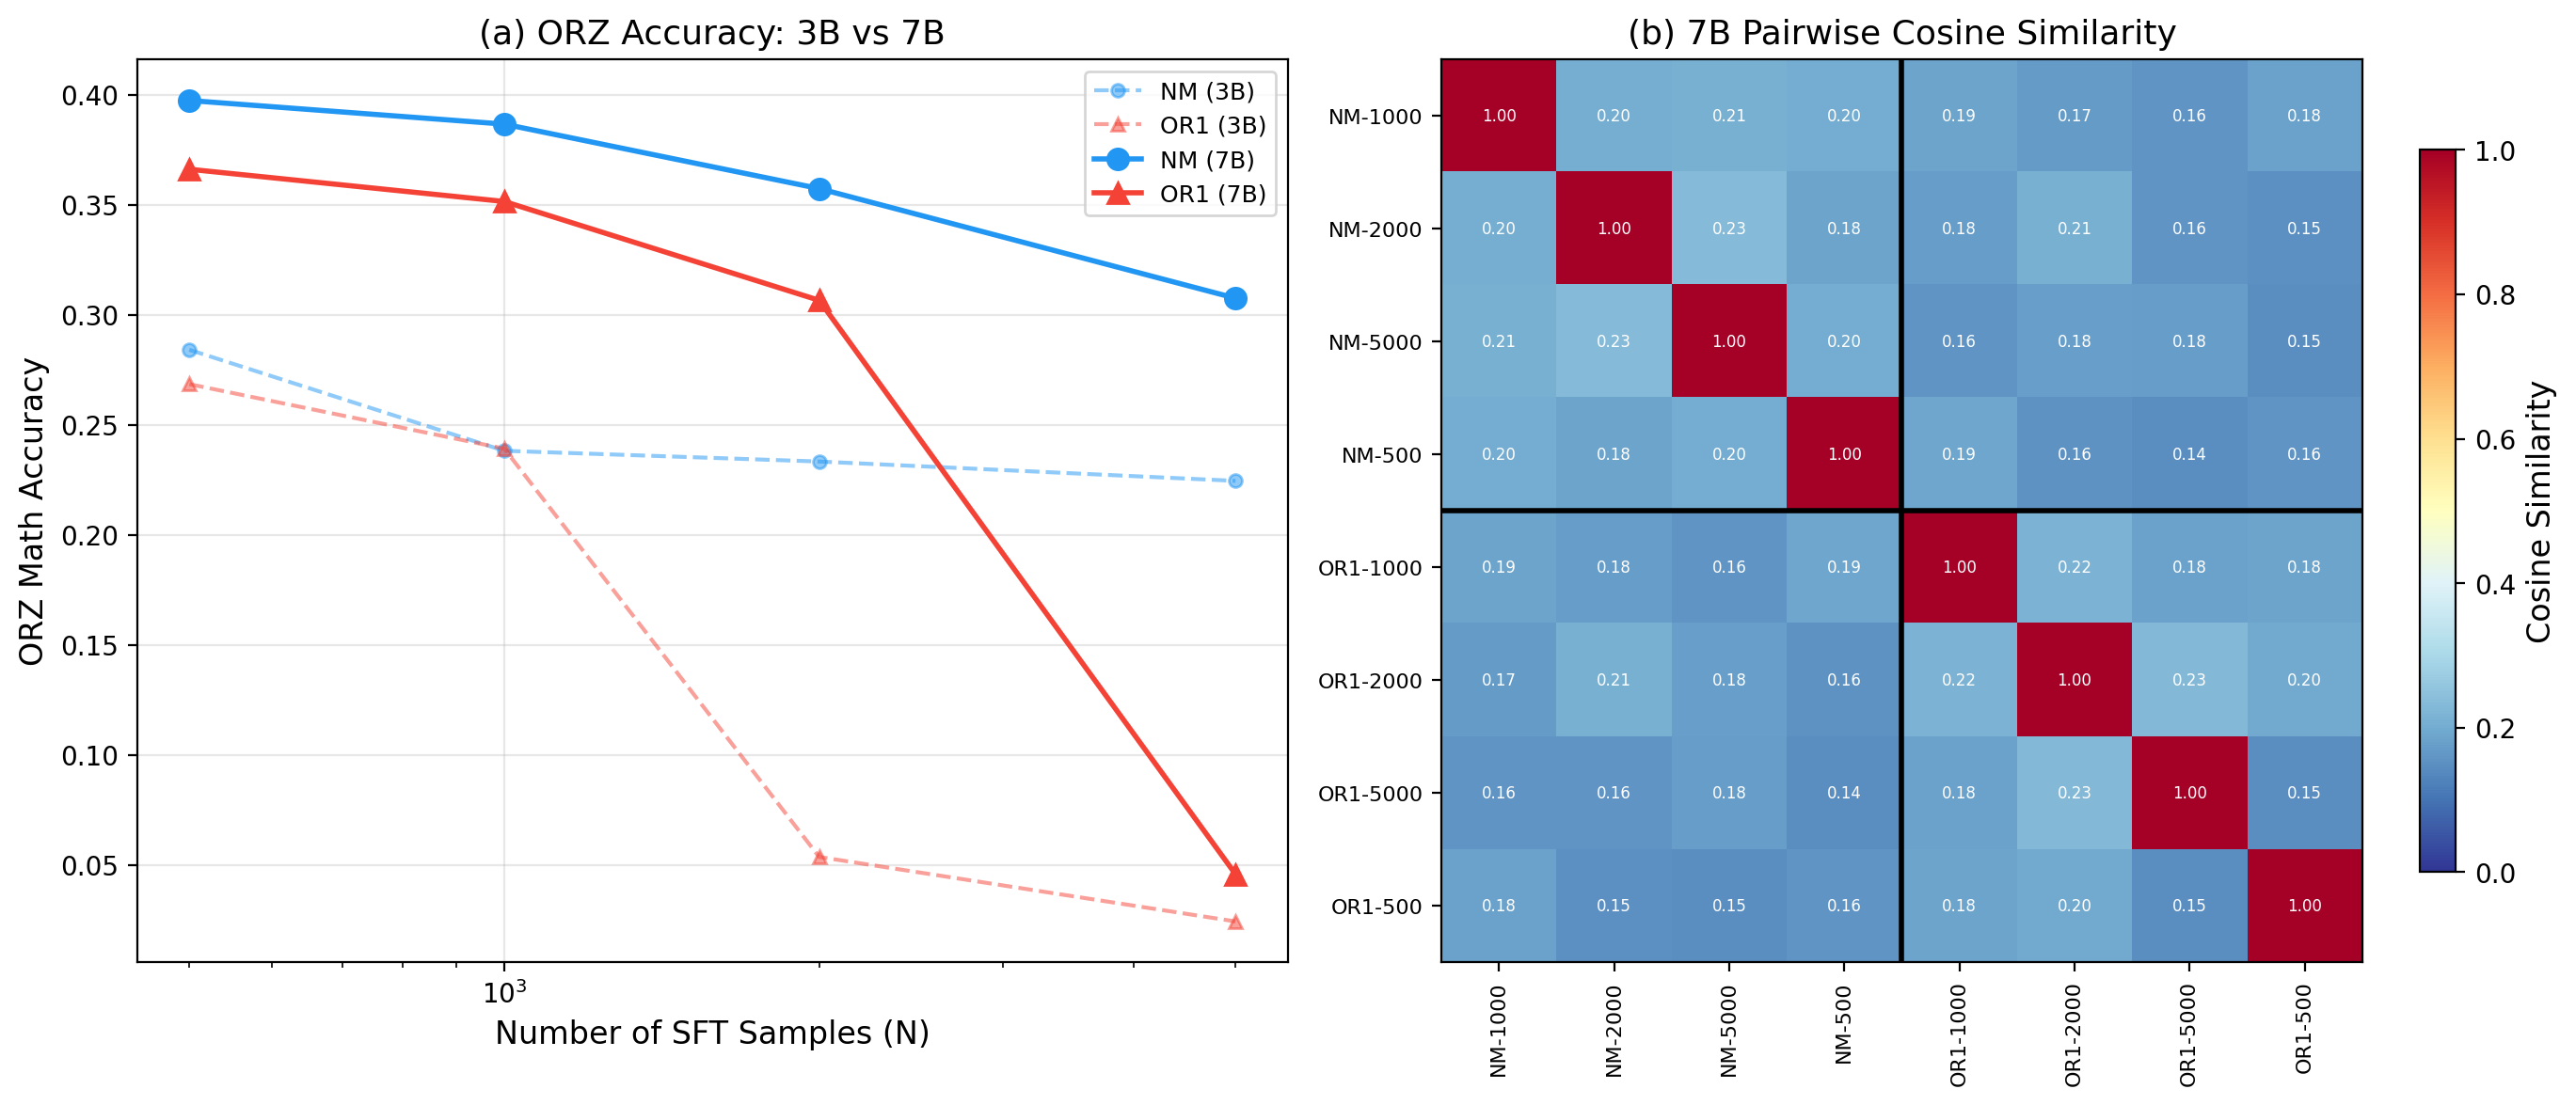
\includegraphics[width=\textwidth]{fig11_7b_comparison.png}
    \caption{7B scale: the OpenR1 cliff shifts to $N{=}5{,}000$ but is qualitatively identical.}
    \label{fig:7b}
\end{subfigure}
\hfill
\begin{subfigure}[t]{0.48\textwidth}
    \centering
    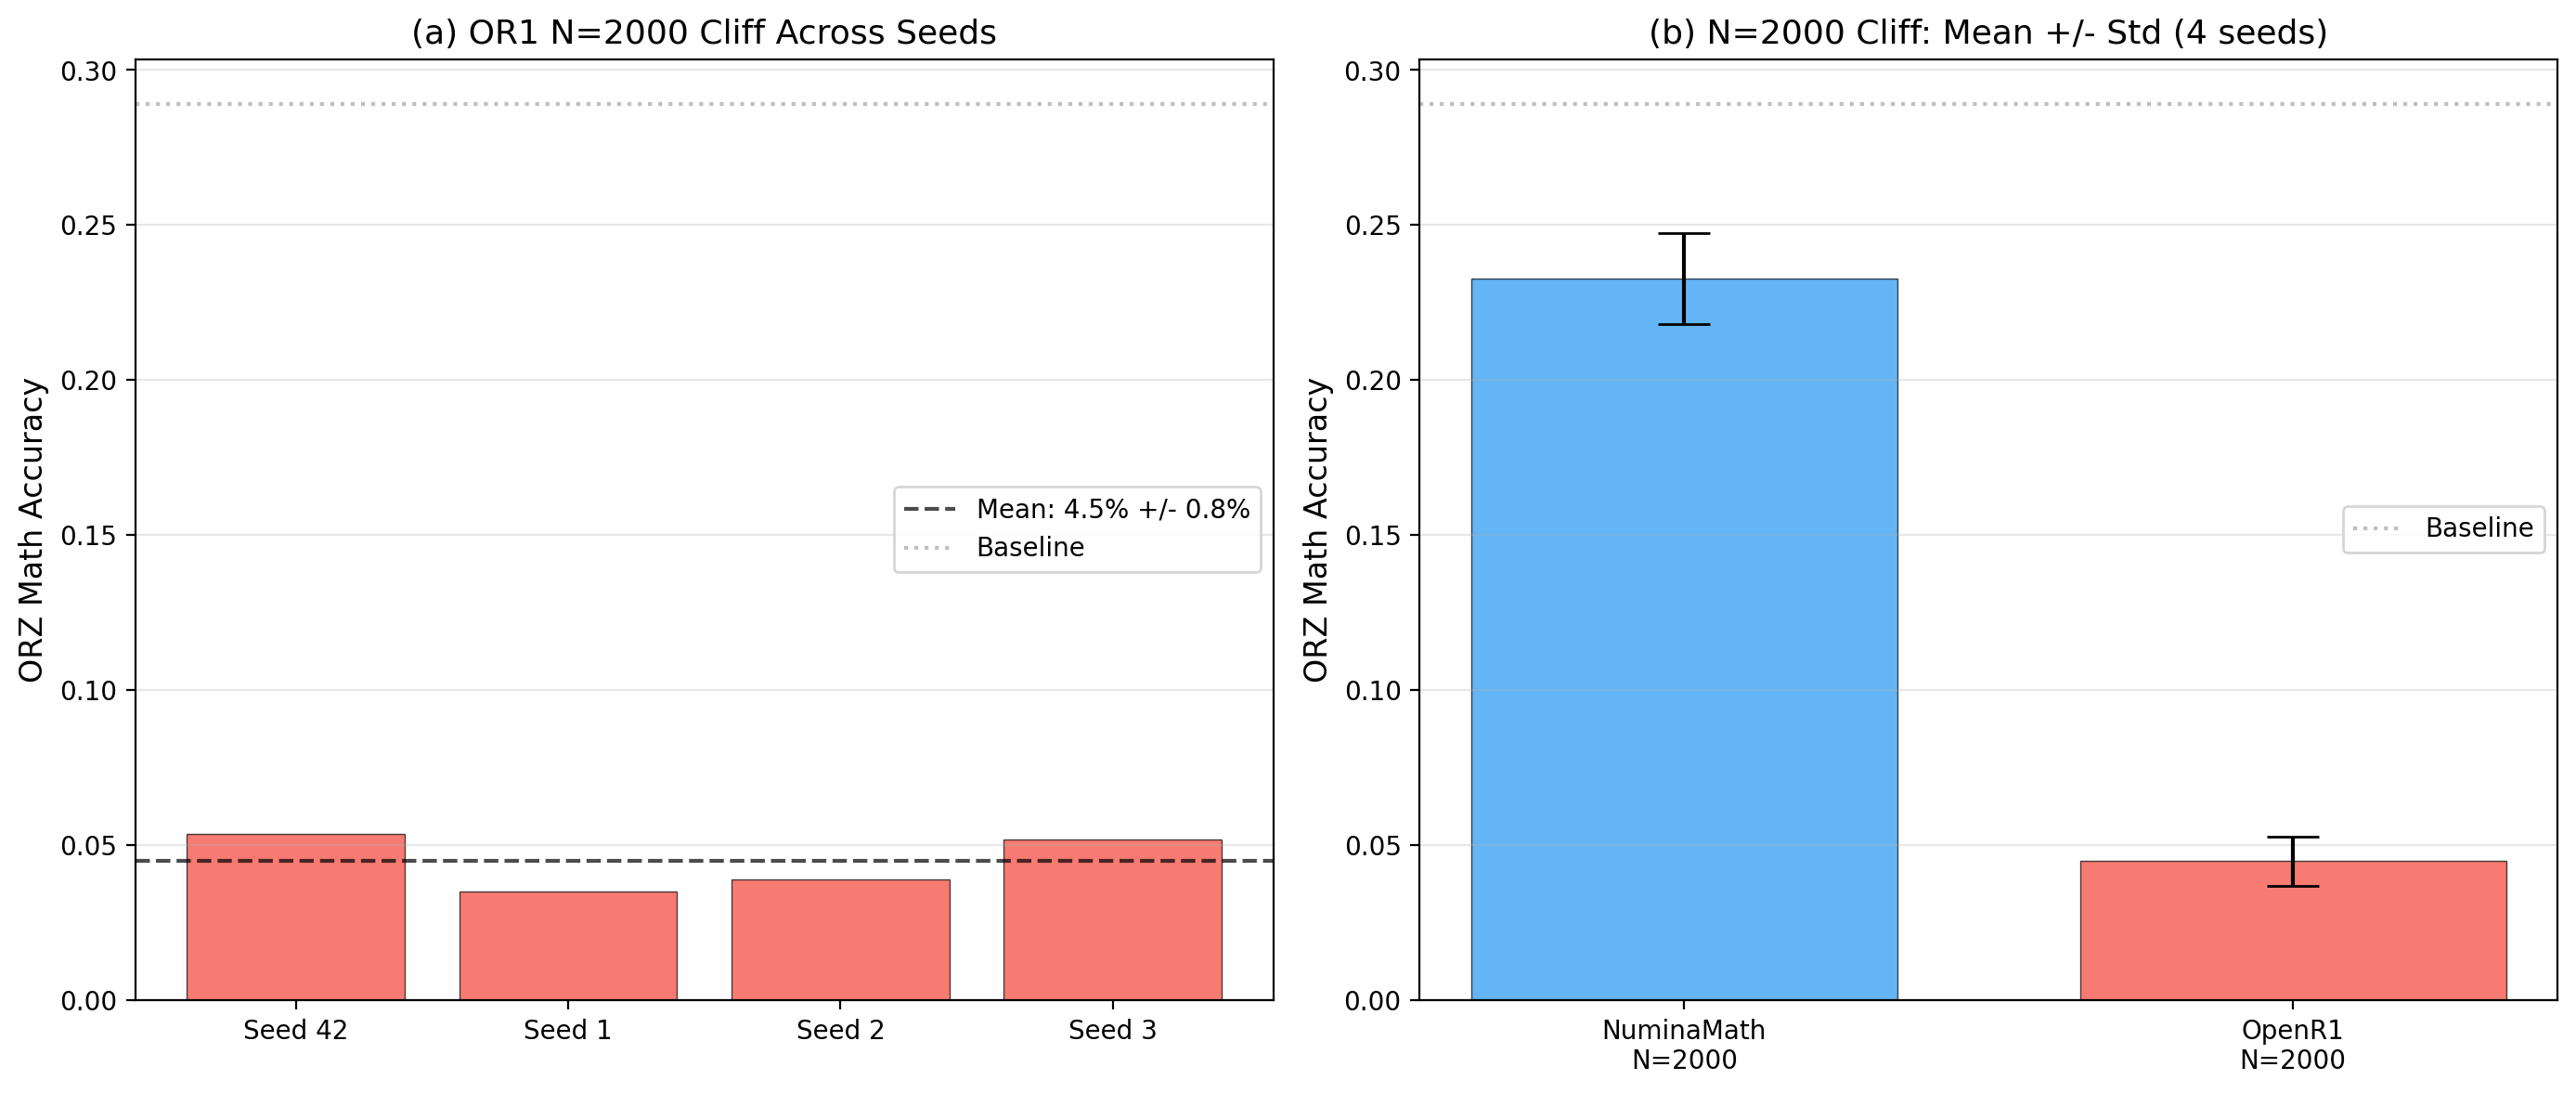
\includegraphics[width=\textwidth]{fig13_cliff_seeds.png}
    \caption{Seed replication at 3B, $N{=}2{,}000$. All seeds collapse; $\sigma = 0.87$\,pp.}
    \label{fig:seeds}
\end{subfigure}
\caption{The phase transition is systematic. (a)~Persists at larger scale with shifted threshold. (b)~Reproduced across random seeds.}
\label{fig:scale-seeds}
\end{figure}

%---------------------------------------------------------------------
\section{Cross-Domain Robustness}
\label{sec:cross-domain}
%---------------------------------------------------------------------

Throughout all 84 experiments, cross-domain benchmarks remain remarkably stable. Even at the height of OpenR1's math collapse ($N{=}10{,}000$, ORZ $= 3.1\%$):

\begin{itemize}
    \item \textbf{SciKnowEval} (chemistry): 27.4\%, degraded but $-$7\,pp is modest relative to the 26\,pp math collapse
    \item \textbf{ToolAlpaca} (tool-use): 89.5\% real func accuracy, \emph{above} the 89.2\% baseline
\end{itemize}

For NuminaMath, cross-domain benchmarks fluctuate within $\pm 3\%$ of baseline across all sample counts, with no systematic trend.

We further test with CodeAlpaca---a non-math SFT source. Code fine-tuning produces the \emph{largest} weight perturbation ($\|\Delta W\|_F = 1.023$ at $N{=}2{,}000$, 1.7$\times$ NuminaMath) yet the \emph{smallest} math degradation ($-$2.2\,pp ORZ). Weight-space cosine similarity between code and math LoRA updates is ${\sim}0.01$ (near-orthogonal), confirming that LoRA perturbations are confined to task-relevant subspaces and format collapse is a within-domain phenomenon.

%---------------------------------------------------------------------
\section{Weight-Space Signatures}
\label{sec:weights}
%---------------------------------------------------------------------

\subsection{Perturbation Magnitude Does Not Explain the Cliff}

A natural hypothesis is that the cliff results from excessive perturbation magnitude. The data refute this:

\begin{table}[h]
\centering
\caption{Matched-norm comparisons. Same $\|\Delta W\|$, vastly different outcomes.}
\label{tab:norm-paradox}
\small
\begin{tabular}{@{}lrrrr@{}}
\toprule
Experiment & $N$ & $\|\Delta W\|_F$ & ORZ Acc. & GSM8K-S \\
\midrule
NuminaMath & 2,000 & 0.60 & 23.3\% & 65.1\% \\
\textbf{OpenR1} & \textbf{2,000} & \textbf{0.79} & \textbf{5.4\%} & \textbf{33.1\%} \\
\midrule
NuminaMath & 10,000 & 0.87 & 20.0\% & 77.0\% \\
OpenR1 & 10,000 & 1.63 & 3.1\% & 50.0\% \\
\midrule
CodeAlpaca & 2,000 & \textbf{1.02} & 26.7\% & -- \\
\bottomrule
\end{tabular}
\end{table}

CodeAlpaca at $\|\Delta W\| = 1.02$ causes less math degradation than OpenR1 at $\|\Delta W\| = 0.79$. NuminaMath at $\|\Delta W\| = 0.87$ maintains $4{\times}$ higher ORZ accuracy than OpenR1 at the smaller $\|\Delta W\| = 0.79$. Perturbation magnitude is necessary but not sufficient to explain the collapse.

\subsection{Directional Divergence}

Computing pairwise cosine similarity between the full weight-update vectors reveals that different data sources push the model in distinct directions in weight space:

\begin{table}[h]
\centering
\caption{Cross-source cosine similarity decreases with $N$, reflecting increasing directional divergence.}
\label{tab:divergence}
\small
\begin{tabular}{@{}rrr@{}}
\toprule
$N$ & NuminaMath vs OpenR1 & NuminaMath vs NM-Hard \\
\midrule
100 & 0.75 & ${\sim}$1.00 \\
500 & 0.75 & ${\sim}$1.00 \\
1,000 & 0.71 & ${\sim}$1.00 \\
2,000 & 0.56 & ${\sim}$1.00 \\
5,000 & 0.36 & 0.93 \\
10,000 & \textbf{0.24} & 0.80 \\
\bottomrule
\end{tabular}
\end{table}

At small $N$, all math sources produce similar perturbation directions (cosine ${\sim}0.75$). As $N$ increases, OpenR1's direction diverges sharply from NuminaMath's (cosine drops to 0.24 at $N{=}10{,}000$). The cliff at $N{\sim}2{,}000$ coincides with the direction cosine dropping below 0.56. NuminaMath and NuminaMath-Hard remain highly aligned at all $N$, consistent with their shared style producing shared weight-space directions.

\begin{figure}[t]
\centering
\begin{subfigure}[t]{0.48\textwidth}
    \centering
    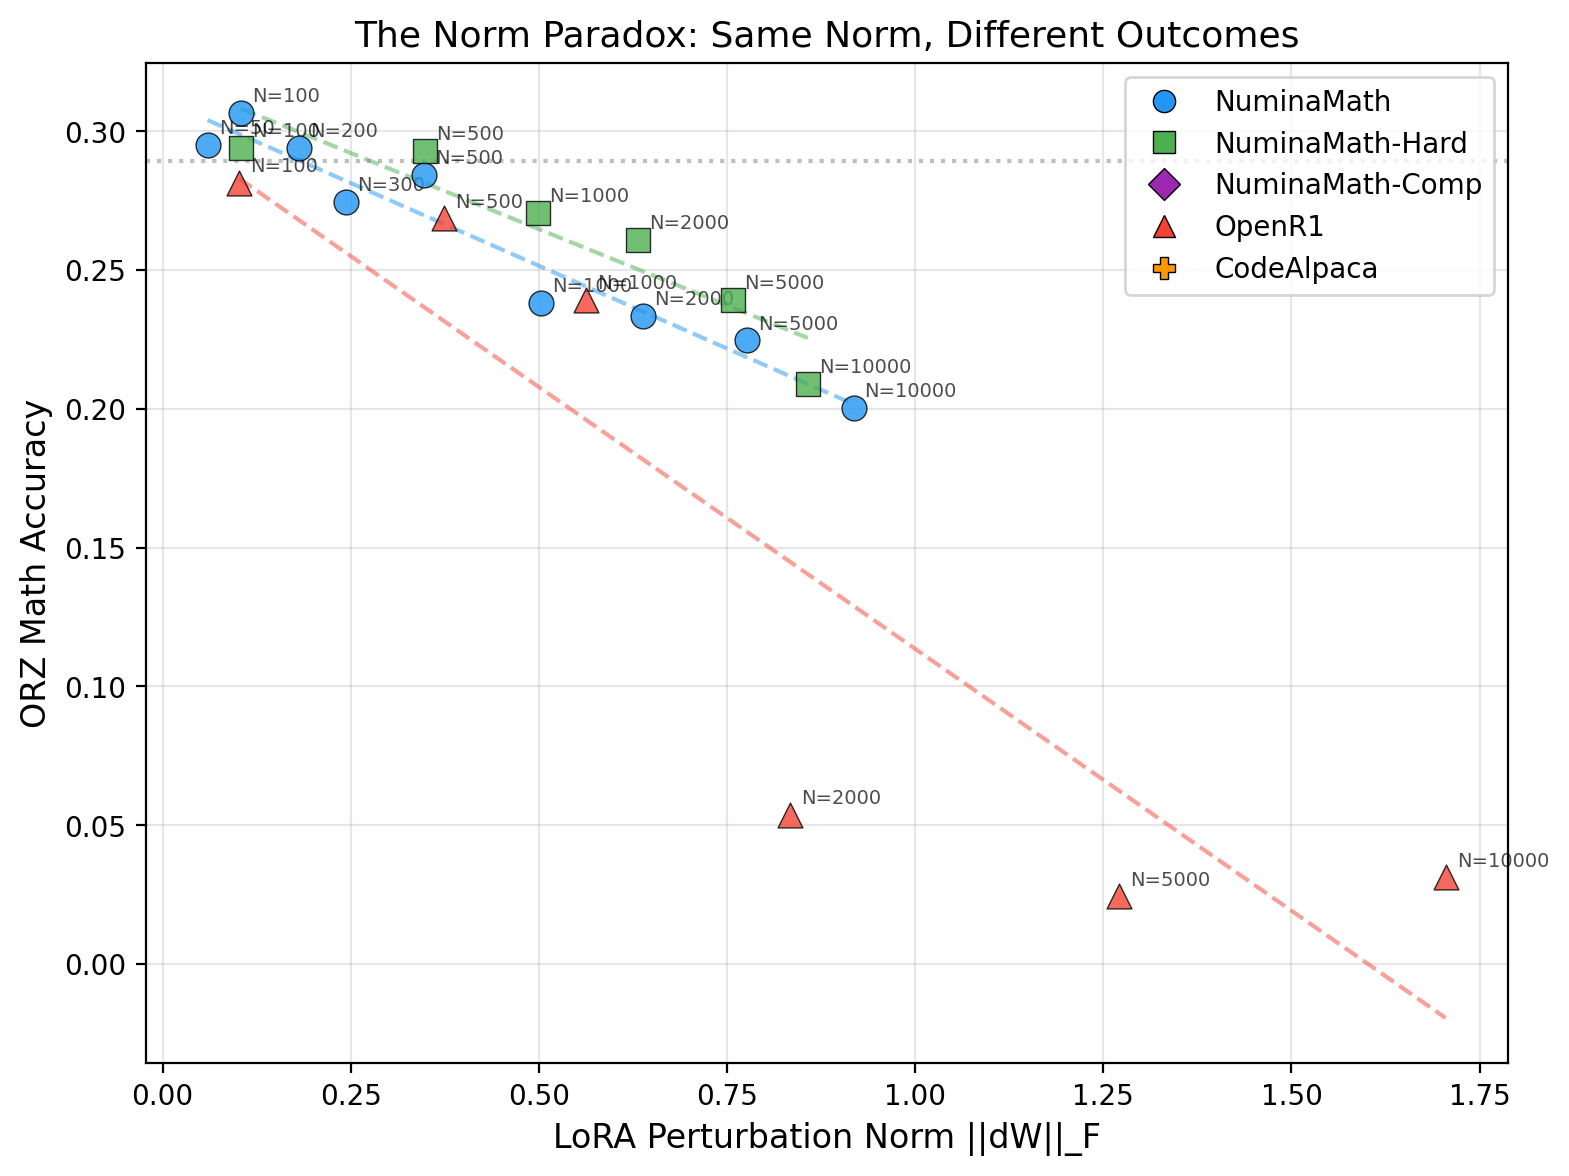
\includegraphics[width=\textwidth]{fig1_norm_vs_orz.png}
    \caption{$\|\Delta W\|_F$ vs.\ ORZ accuracy. Same norm, different outcomes across sources.}
    \label{fig:norm}
\end{subfigure}
\hfill
\begin{subfigure}[t]{0.48\textwidth}
    \centering
    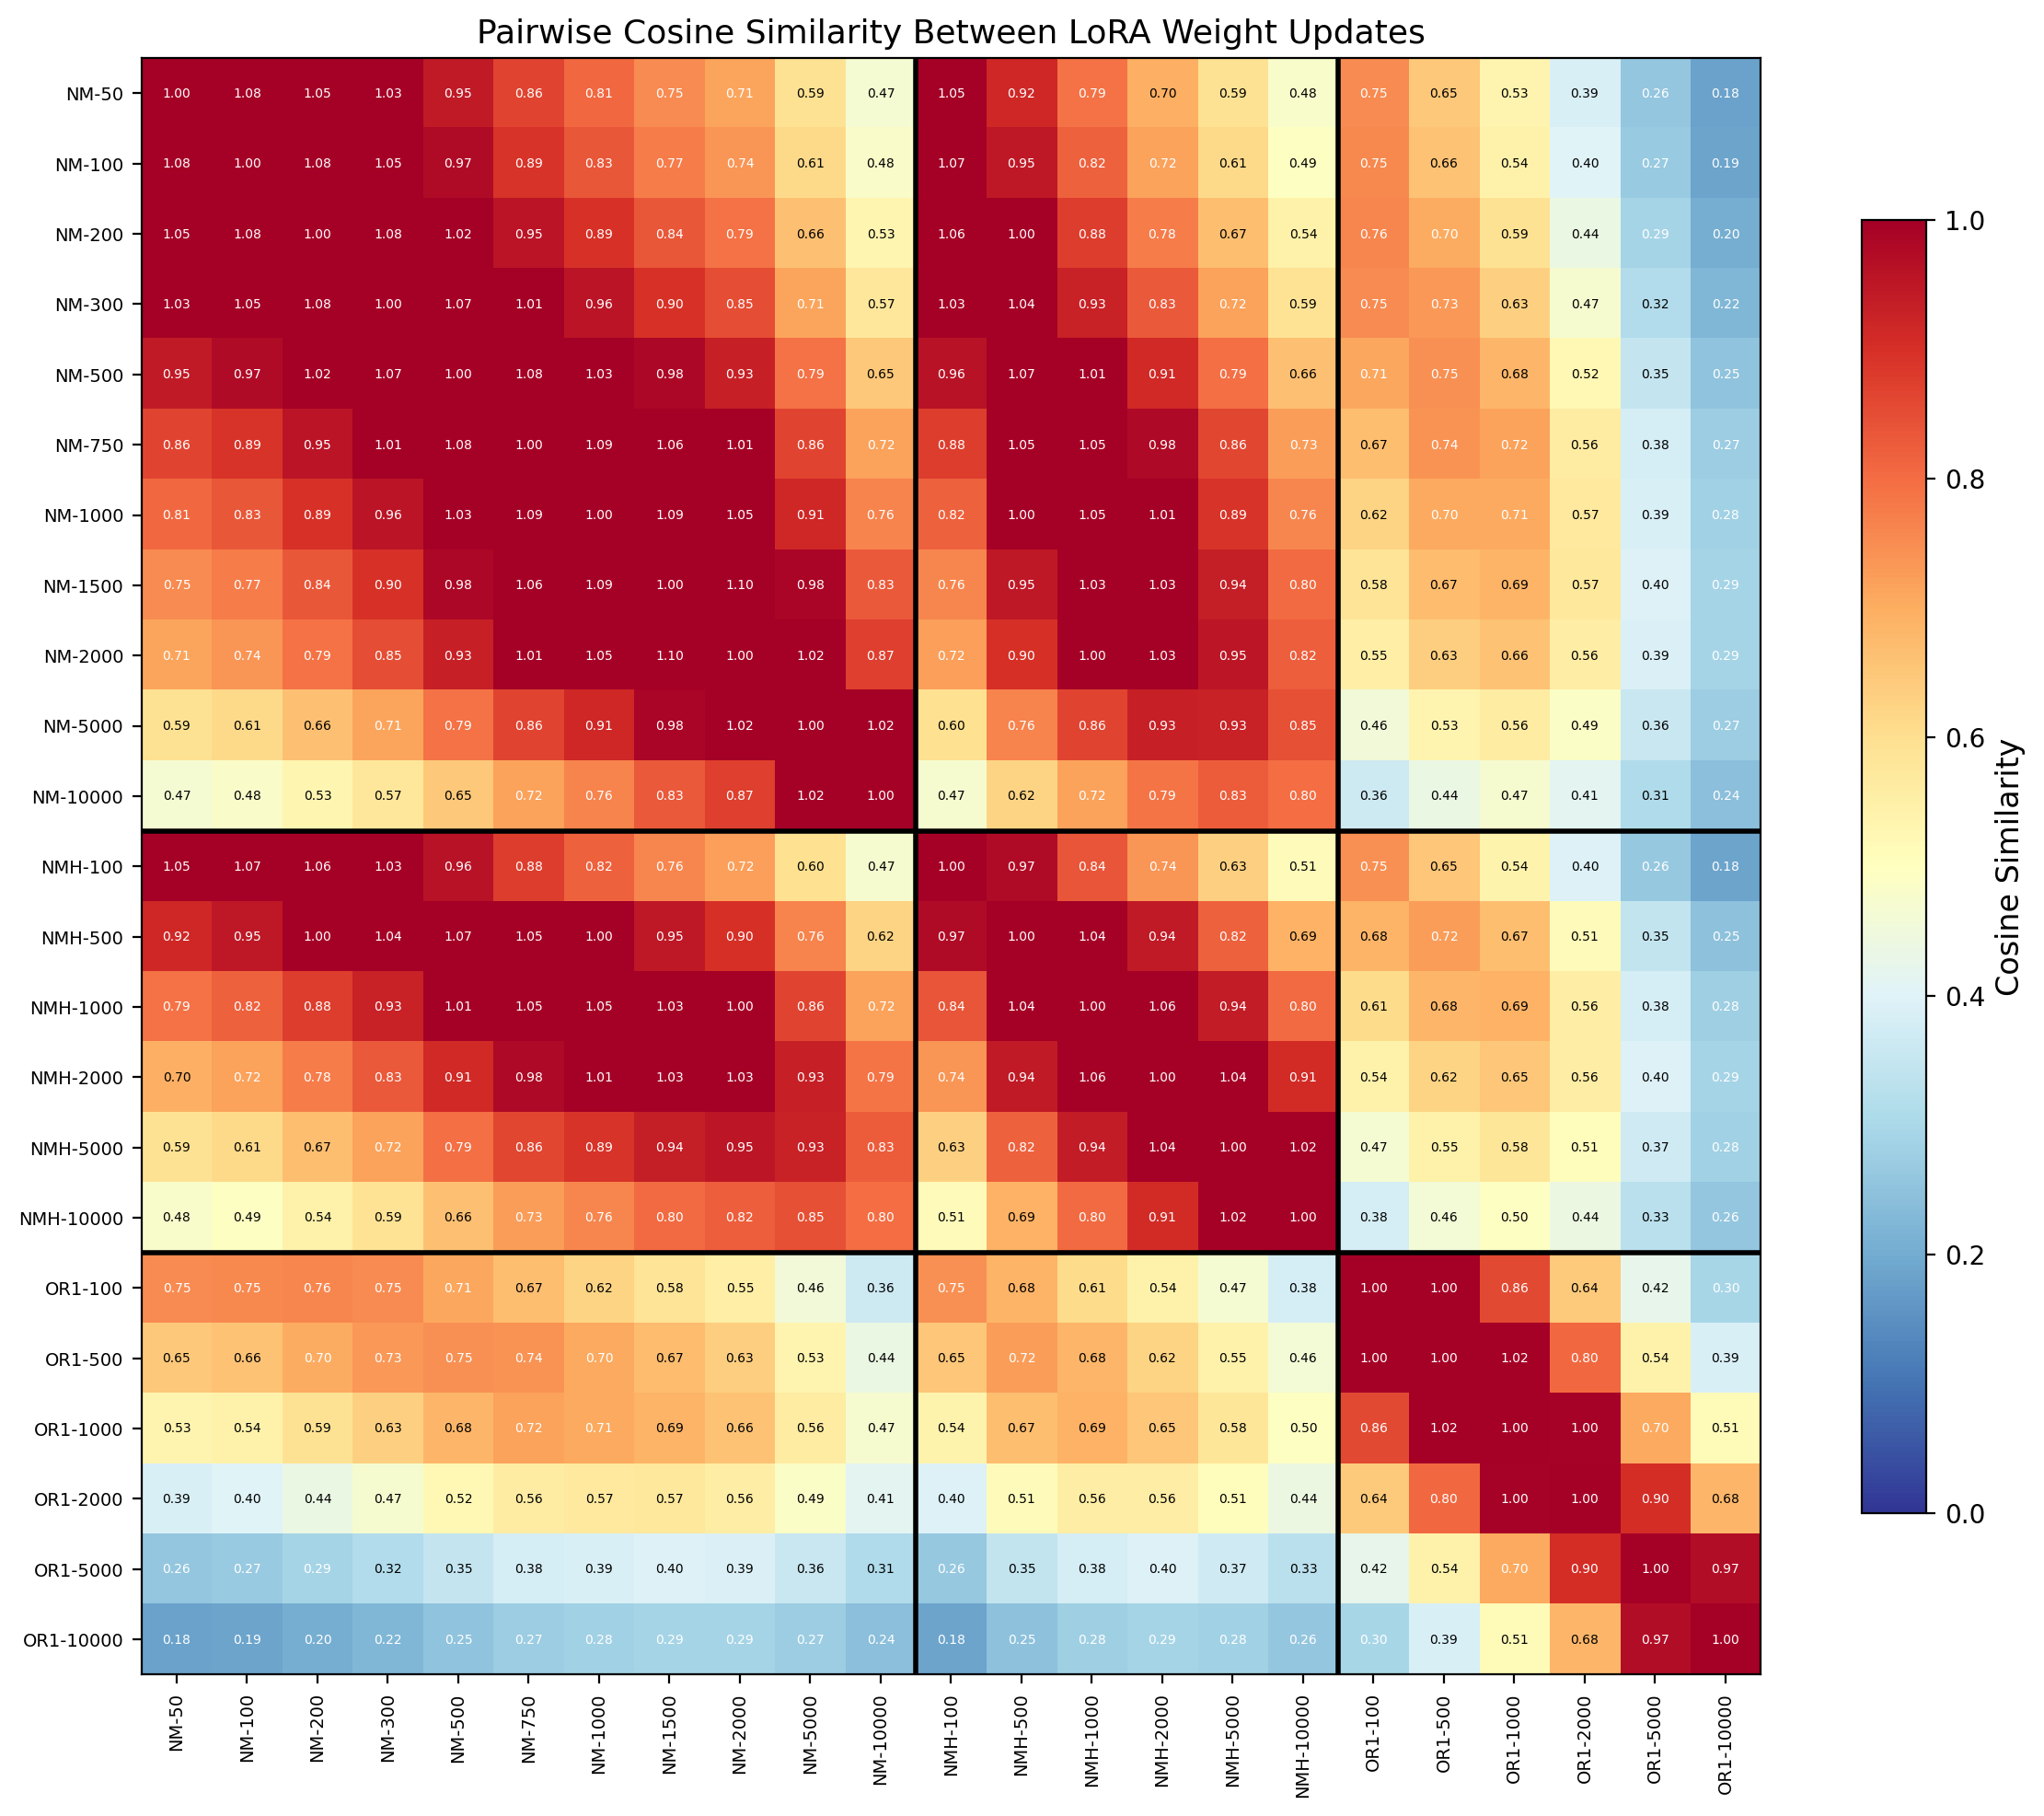
\includegraphics[width=\textwidth]{fig2_cosine_heatmap.png}
    \caption{Cosine similarity heatmap. Block structure reveals source-dependent directions.}
    \label{fig:heatmap}
\end{subfigure}
\caption{Weight-space analysis. (a)~Norm alone does not predict degradation across sources. (b)~LoRA updates cluster by data source, with increasing divergence at higher $N$.}
\label{fig:weights}
\end{figure}

%---------------------------------------------------------------------
\section{Discussion}
\label{sec:discussion}
%---------------------------------------------------------------------

\subsection{Why a Phase Transition?}

The sharpness of the OpenR1 cliff suggests a threshold mechanism rather than gradual accumulation. We hypothesize that the model maintains two competing ``modes''---its original concise instruction-following mode and the verbose R1-style mode being trained in. At low $N$, the original mode dominates. At the critical $N$, the verbose mode wins and the model's default generation strategy flips. This is consistent with:

\begin{itemize}
    \item The discontinuity (no intermediate behavior between 83\% and 33\%)
    \item The response length jump (mode switch from concise to verbose)
    \item The format compliance cliff (mode switch from structured to free-form)
    \item The mixing threshold (50\% verbose data is tolerated; 75\% is not)
\end{itemize}

\subsection{Why Does Concise Data Self-Correct?}

NuminaMath's transient format disruption at $N{=}1{,}000$ followed by recovery is puzzling. We propose that all math SFT disrupts formatting conventions during early training (the model is ``relearning'' how to present solutions). With concise data, the training examples themselves demonstrate the correct format, so continued training reinforces it. With verbose data, the training examples demonstrate a fundamentally different format, so continued training reinforces the wrong conventions.

This explains the asymmetry: format disruption is universal, but recovery requires format-compatible training data.

\subsection{Practical Implications}

\textbf{For R1-style distillation.} The growing practice of distilling long-chain reasoning from R1-style models carries a hidden risk: catastrophic format collapse at moderate training volumes. This risk is invisible to tolerant evaluation and only surfaces under strict formatting requirements---which are standard in math benchmarks and production systems.

\textbf{Mitigations.} Our results suggest several practical strategies:
\begin{enumerate}
    \item \textbf{Length budgeting}: truncate verbose solutions to bounded length before SFT.
    \item \textbf{Format anchoring}: mix verbose data with concise, format-compliant examples (${\leq}50\%$ verbose appears safe).
    \item \textbf{Monitoring}: track strict vs.\ tolerant accuracy and response length during training to detect early signs of style transfer.
    \item \textbf{Scale-aware budgets}: larger models tolerate more verbose data; the safe $N$ scales with model capacity.
\end{enumerate}

%---------------------------------------------------------------------
\section{Limitations}
%---------------------------------------------------------------------

\textbf{Two model scales.} We test on Qwen2.5 at 3B and 7B. Whether the phase transition exists in much larger models (70B+), and whether the scaling relationship holds, is unknown.

\textbf{Single model family.} All experiments use Qwen2.5. Other architectures may have different vulnerability profiles.

\textbf{Limited domain diversity.} We establish the phenomenon for math reasoning with a code control. Whether verbose training data causes format collapse in other domains (summarization, dialogue) requires further study.

\textbf{Mechanism is descriptive.} We characterize the transition and identify verbosity as the driver but do not provide a mechanistic explanation at the level of attention heads or circuits.

%---------------------------------------------------------------------
\section{Conclusion}
%---------------------------------------------------------------------

We have identified \textbf{catastrophic format collapse}: a sharp phase transition in LoRA fine-tuning where output formatting fails while reasoning capability persists. The transition is:

\begin{itemize}
    \item \textbf{Sharp}: 500 samples cause a 50\,pp accuracy drop
    \item \textbf{Reproducible}: $\sigma = 0.87$\,pp across 4 seeds
    \item \textbf{Caused by verbosity}: truncating training data recovers 50\% of lost accuracy
    \item \textbf{Scale-dependent}: threshold shifts from $N{\sim}1{,}500$ (3B) to $N{\sim}5{,}000$ (7B)
    \item \textbf{Asymmetric}: concise data causes transient disruption that self-corrects; verbose data causes permanent collapse
\end{itemize}

The core insight is that \textbf{SFT transfers style, not just knowledge}. When the style of training data is sufficiently different from the model's baseline, the model's output conventions collapse before its reasoning does. This has direct implications for the widespread practice of R1-style distillation: verbose training data improves reasoning chains but, beyond a critical volume, catastrophically destroys the formatting that makes those chains evaluable.

Standard evaluation practices conflate format compliance with reasoning ability. Separately tracking these two dimensions---as our strict/tolerant decomposition demonstrates---is essential for understanding what SFT actually does to a model.

%---------------------------------------------------------------------
\bibliographystyle{plainnat}

\begin{thebibliography}{10}

\bibitem[Biderman et~al.(2024)]{biderman2024lora}
D.~Biderman, J.~Portes, J.~G.~Ortiz, M.~Greber, G.~L.~Doney, S.~Shahsavari, H.~Patel, K.~Scheible, C.~Kacmarcik, and L.~Hestness.
\newblock {LoRA} learns less and forgets less.
\newblock \emph{arXiv:2405.09673}, 2024.

\bibitem[Chen et~al.(2023)]{chen2023alpagasus}
L.~Chen, S.~Li, J.~Yan, H.~Wang, K.~Gunaratna, V.~Yadav, Z.~Tang, V.~Srinivasan, T.~Zhou, H.~Huang, and H.~Jin.
\newblock {AlpaGasus}: Training a better {Alpaca} with fewer data.
\newblock \emph{arXiv:2307.08701}, 2023.

\bibitem[Hu et~al.(2022)]{hu2022lora}
E.~J.~Hu, Y.~Shen, P.~Wallis, Z.~Allen-Zhu, Y.~Li, S.~Wang, L.~Wang, and W.~Chen.
\newblock {LoRA}: Low-rank adaptation of large language models.
\newblock In \emph{ICLR}, 2022.

\bibitem[Kirkpatrick et~al.(2017)]{kirkpatrick2017overcoming}
J.~Kirkpatrick, R.~Pascanu, N.~Rabinowitz, J.~Veres, G.~Desjardins, A.~A.~Rusu, K.~Milan, J.~Quan, T.~Ramalho, A.~Grabska-Barwinska, et~al.
\newblock Overcoming catastrophic forgetting in neural networks.
\newblock \emph{PNAS}, 114(13), 2017.

\bibitem[Li et~al.(2024)]{li2024numinamath}
Y.~Li et~al.
\newblock {NuminaMath}: A large-scale curated dataset for mathematical reasoning, 2024.

\bibitem[Luo et~al.(2023)]{luo2023empirical}
Y.~Luo, Z.~Yang, F.~Meng, Y.~Li, J.~Zhou, and Y.~Zhang.
\newblock An empirical study of catastrophic forgetting in large language models during continual fine-tuning.
\newblock \emph{arXiv:2308.08747}, 2023.

\bibitem[{Open-Reasoner}(2024)]{openr1}
{Open-Reasoner}.
\newblock {OpenR1-Math}: High-quality math reasoning data from {R1} distillation, 2024.

\bibitem[Yang et~al.(2024)]{yang2024qwen}
A.~Yang et~al.
\newblock {Qwen2.5} technical report.
\newblock \emph{arXiv:2412.15115}, 2024.

\bibitem[Zhou et~al.(2023)]{zhou2023lima}
C.~Zhou, P.~Liu, P.~Xu, S.~Iyer, J.~Sun, Y.~Mao, X.~Ma, A.~Efrat, P.~Yu, L.~Yu, S.~Zhang, G.~Ghosh, M.~Lewis, L.~Zettlemoyer, and O.~Levy.
\newblock {LIMA}: Less is more for alignment.
\newblock In \emph{NeurIPS}, 2023.

\end{thebibliography}

%---------------------------------------------------------------------
\newpage
\appendix
\section{Complete Experimental Results}
\label{app:results}

\subsection{NuminaMath Standard Config ($r{=}8$, LR$=5{\times}10^{-5}$, 1 epoch)}

\begin{table}[h]
\centering
\small
\begin{tabular}{@{}rrrrrrr@{}}
\toprule
$N$ & ORZ & $\|\Delta W\|_F$ & SciKnow & TA-Real F & GSM8K-S & Valid \\
\midrule
50 & 29.5\% & 0.056 & 34.0\% & 89\% & -- & Y \\
100 & 30.7\% & 0.098 & 35.2\% & 89\% & 83.6\% & Y \\
200 & 29.4\% & 0.172 & 33.4\% & 89\% & -- & Y \\
300 & 27.4\% & 0.230 & 33.8\% & 89\% & -- & Y \\
500 & 28.4\% & 0.330 & 35.3\% & 89\% & 82.7\% & Y \\
750 & 26.9\% & 0.410 & 31.9\% & 89\% & -- & Y \\
1,000 & 23.8\% & 0.478 & 32.6\% & 88\% & 62.9\% & Y \\
1,500 & 22.0\% & 0.551 & 32.0\% & 89\% & -- & Y \\
2,000 & 23.3\% & 0.604 & 31.6\% & 89\% & 65.1\% & Y \\
5,000 & 22.5\% & 0.733 & 33.8\% & 91\% & 75.5\% & Y \\
10,000 & 20.0\% & 0.869 & 31.5\% & 90\% & 77.0\% & Y \\
\bottomrule
\end{tabular}
\end{table}

\subsection{OpenR1 Standard Config}

\begin{table}[h]
\centering
\small
\begin{tabular}{@{}rrrrrrr@{}}
\toprule
$N$ & ORZ & $\|\Delta W\|_F$ & SciKnow & TA-Real F & GSM8K-S & Valid \\
\midrule
100 & 28.1\% & 0.096 & 34.6\% & 89\% & 84.2\% & Y \\
500 & 26.9\% & 0.356 & 34.9\% & 88\% & 83.4\% & Y \\
1,000 & 23.9\% & 0.529 & 33.7\% & 86\% & 77.2\% & N \\
1,250 & 25.7\% & 0.445 & 33.4\% & 89\% & 83.5\% & Y \\
1,500 & 25.9\% & 0.489 & 32.0\% & 87\% & 83.0\% & Y \\
\textbf{2,000} & \textbf{5.4\%} & \textbf{0.789} & 35.8\% & 86\% & \textbf{33.1\%} & N \\
5,000 & 2.4\% & 1.211 & 30.1\% & 89\% & 33.7\% & N \\
10,000 & 3.1\% & 1.628 & 27.4\% & 89\% & 50.0\% & N \\
\bottomrule
\end{tabular}
\end{table}

\subsection{NuminaMath Seed Variations}

\begin{table}[h]
\centering
\small
\caption{NuminaMath seed variations (standard config, 4 seeds each).}
\begin{tabular}{@{}rrrr@{}}
\toprule
$N$ & ORZ Mean $\pm$ Std & Range & Seed Variance \\
\midrule
100 & 29.6\% $\pm$ 1.0 & 28.5--30.7\% & Low \\
500 & 28.4\% $\pm$ 0.2 & 28.0--28.6\% & Very low \\
2,000 & 22.6\% $\pm$ 0.5 & 22.2--23.3\% & Low \\
10,000 & 19.9\% $\pm$ 0.5 & 19.0--20.5\% & Low \\
\bottomrule
\end{tabular}
\end{table}

\subsection{CodeAlpaca (Non-Math Control)}

\begin{table}[h]
\centering
\small
\begin{tabular}{@{}rrrrrr@{}}
\toprule
$N$ & ORZ & $\|\Delta W\|_F$ & SciKnow & TA-Real F & Valid \\
\midrule
500 & 29.4\% & 0.581 & 33.9\% & 89\% & Y \\
1,000 & 29.3\% & 0.826 & 34.4\% & 90\% & Y \\
2,000 & 26.7\% & 1.023 & 31.5\% & 89\% & Y \\
5,000 & 24.4\% & 1.151 & 33.1\% & 89\% & Y \\
\bottomrule
\end{tabular}
\end{table}

\end{document}
